% !TEX TS–program = pdflatexmk
\documentclass[conference]{article}
\usepackage{times}
\usepackage{amsmath}
\usepackage{gensymb}
% numbers option provides compact numerical references in the text.
\usepackage[numbers]{natbib}
\usepackage{multicol}
\usepackage[bookmarks=true]{hyperref}

\usepackage{graphicx}

\pdfinfo{
   /Author (Homer Simpson)
   /Title  (Robots: Our new overlords)
   /CreationDate (D:20101201120000)
   /Subject (Robots)
   /Keywords (Robots;Overlords)
}

\begin{document}

% paper title
\title{Controlling a Variable Geometry Truss Tetrobot with an Isomporphic Puppet Controller}

% You will get a Paper-ID when submitting a pdf file to the conference system
\author{Author Names Omitted for Anonymous Review. Paper-ID [add your ID here]}



\maketitle

\begin{abstract}
  Humans are skillful.
  By building a bio-inspired manipulable snake-like controller that can be
  molded into a wide variety of shapes, we allow a human controller to telepresently
  specify complex shapes and shape changes.
  We constructed a tetrahelix consisting of seven tetrahedron made of
  adjustable-length members connected via 3D printed Song-Kwon-Kim joints which
  allow manual changes to the shape of the controller. These changes in length are
  digitized and organized via an Arduino and transmitted to more power computers
  where they may specify a shape to be animated or control a robot of similar shape,
  or simply specify relative positions in Cartesian space. Although this research is basic,
  we hope it will eventually amplify human control of in vivo mechanical devices such as
  endoscopes, search-and-rescue robots weaseling into tight spaces, or general purpose
  tetrobots used for planetary space exploration as suggested by
  Prof. Sanderson and his students 20 years ago.
\end{abstract}



\section{Introduction}

The possibility of building a robot based on tetrahedra constructed of
tensegrities has been well researched \citet{TetrobotBook,NTRT,paul2006,chen2017soft}.
It is possible to construct a variable geometry truss out of actuators
using tetrahedra as a repeated module that might be expected to have
an advantageous strength-to-weight ratio \citet{mikulas1985sequentially,mirletz2014}.
The existence of the Boerdijk-Coxeter tetrahelix \citet{coxeter1985simplicial}
has long been recognized \citet{fuller1982synergetics,graytetrahelix} as a
geometric means of composing tetrahedra into long beam, which
might combine the structural advanatages of a tetrahedral tensegrity with
snake-like robot motion \citet{hirose1993biologically,liljebäck2012snake}.

By utilizing a 3D-printed jointing system
 which
 supports angular displacement of multiple members coming to central point
 extending previously patented work \citet{song2003spherical} and small-scale
 actuators and microcontrollers, the authors have constructed a relatively
 inexpensive tetrobot. Although some headway has been made in numerical
 control, this papers explores the fundamental idea of using a simulacrum
 controller. A controller which is isomporphic to the robot (but smaller)
 is constructed
 which can be manipulated by hand by an operated. The larger robots mimics
 the motion of the controller. This controller, called the {\em tetrocon},
 has been used to develop a better hexapodal walking and turning gaits
 than previously possible for the tetrobot. Striking an object in space
 with the end effector is easy with the controller. The controller even allows, with some effort,
 locomotion around or over obstacles.  This paper reports on the tetrocon
 and its usage.

 Although developed to control the tetrobot, the controller could be used
 independently as a shape-input device. For example, it could control
 a tentacle animation or, more importantly, a surgical robot that had
 basically snake-like or
 tentacle-like properties, such as an advanced endoscope or arthroscope.

 \section{Design and Manufacture}

 All hardware and software the designs of the controller are free-libre
 open source \citet{anonymous}.

 A tensegrity is a device in which each member only supports and has to
 support either tensile or compressive loads, or both.
 No member has to resist angular displacement.
 Tensegrities usually use cables for the tensile compoments and rods
 for the compessive components. Tensegrity robots vary the length of one or
 the other.
 Since a cable attached to a point can pull in any direction, the tensegrity
 condition is achieved by attaching rods only to cables, not other rods.

  However, \citet{HamlinSandersonCMS} produced a novel concentric
  multilink spherical joint based on parallelograms. Such joints allow the
  construction of tensegrities without cables (or, equivalently, where the
  cable length has shrunk to zero.)

 \subsection{The Song-Kwon-Kim Concentric Multimember Joint}

 Somewhat later
 \citet{song2003spherical} patented a modification of a ball-and-socket
 joint which is roughly similar. 3D printing makes the construction of
 Song-Kwon-Kim joint practical and inexpensive, though it is not necssarily
 superior.

 Such joints allow multiple rods to be connected with spherical rotation
 around a single point, automatically forming a tensegrity.
 If those rods can change length on their own power, they form a
 machine or robot. If those rods can be changed by external forces,
 the form an input device.
 If you build both, you can have robot \ref{fig:7tetrobot} which mimics a simulacrum or
 puppet controller \ref{fig:7tetrocontroller} you can shape with your hands.

 \subsection{The Lock Component Designed for a Tetrahelix}

 In a Song-Kwon-Kim style joint, a spherical lock holds rotors in place. The placement of
 the holes for the rotors depends on the geometry of the robot one is trying to create.
 For tetrahedral tensegrities wherein the the ratio of the maximum length of an actuator to the
 minimum does not exceed the inverse of the golden ratio, the holes can be placed so
 that all configurations are possible. That is, the robot can never break itself by
 attempting to move into an unattainable configuration.


 \begin{figure}
  \centering
  \includegraphics[width=0.5\textwidth]{figures/JointAssemblyWithRotor.png}
    \caption[Exploded view of Song-Kwon-Kim Joint]{Exploded view of Song-Kwon-Kim Joint}
      \label{fig:JointAssemblyWithRotor}
\end{figure}

 This relies on making the spherical part of the rotor in contact with the ball triangle.
 Making the the rotor trianglular lets the hole the shaft penetrates be made larger,
 allowing a greater angular displacement. So long as the rotors can revolve, then in
 the tighter configuration the rotors meet edge-to-edge.  This has the further advantage
 of strenthenging the points of contact with the lock when in tension.

 \subsection{A Universal Rotor}


 \begin{figure}
  \centering
  \includegraphics[width=0.5\textwidth]{figures/UniversalRotor.png}
    \caption[A Universal Rotor with a Triangular Face]{A Universal Rotor with a Triangular Face}
      \label{fig:UniversalController}
\end{figure}

 Early prototypes of our version of the joint connected the actuator to a rotor in a way
 that was difficult to disconnect. We have replaced this with a standard, or universal,
 rotor shape. The universal rotor has a hole which allows it to be detached from the
 sensor or actuator connected to it by removing a zip tie or a bolt.

 The result is that the joint itself does not have to be taken apart to repair an actuator
 or displacement sensor.
 This has been a great help in the maintenance of the robot.

 In our construction of the robot, we found it necessary to make some pieces of the joint
 out of metal, whereas on the smaller and less force-oriented scale of the controller the
 same parts were servicable when 3D printed in plastic.






\begin{figure}
  \centering
  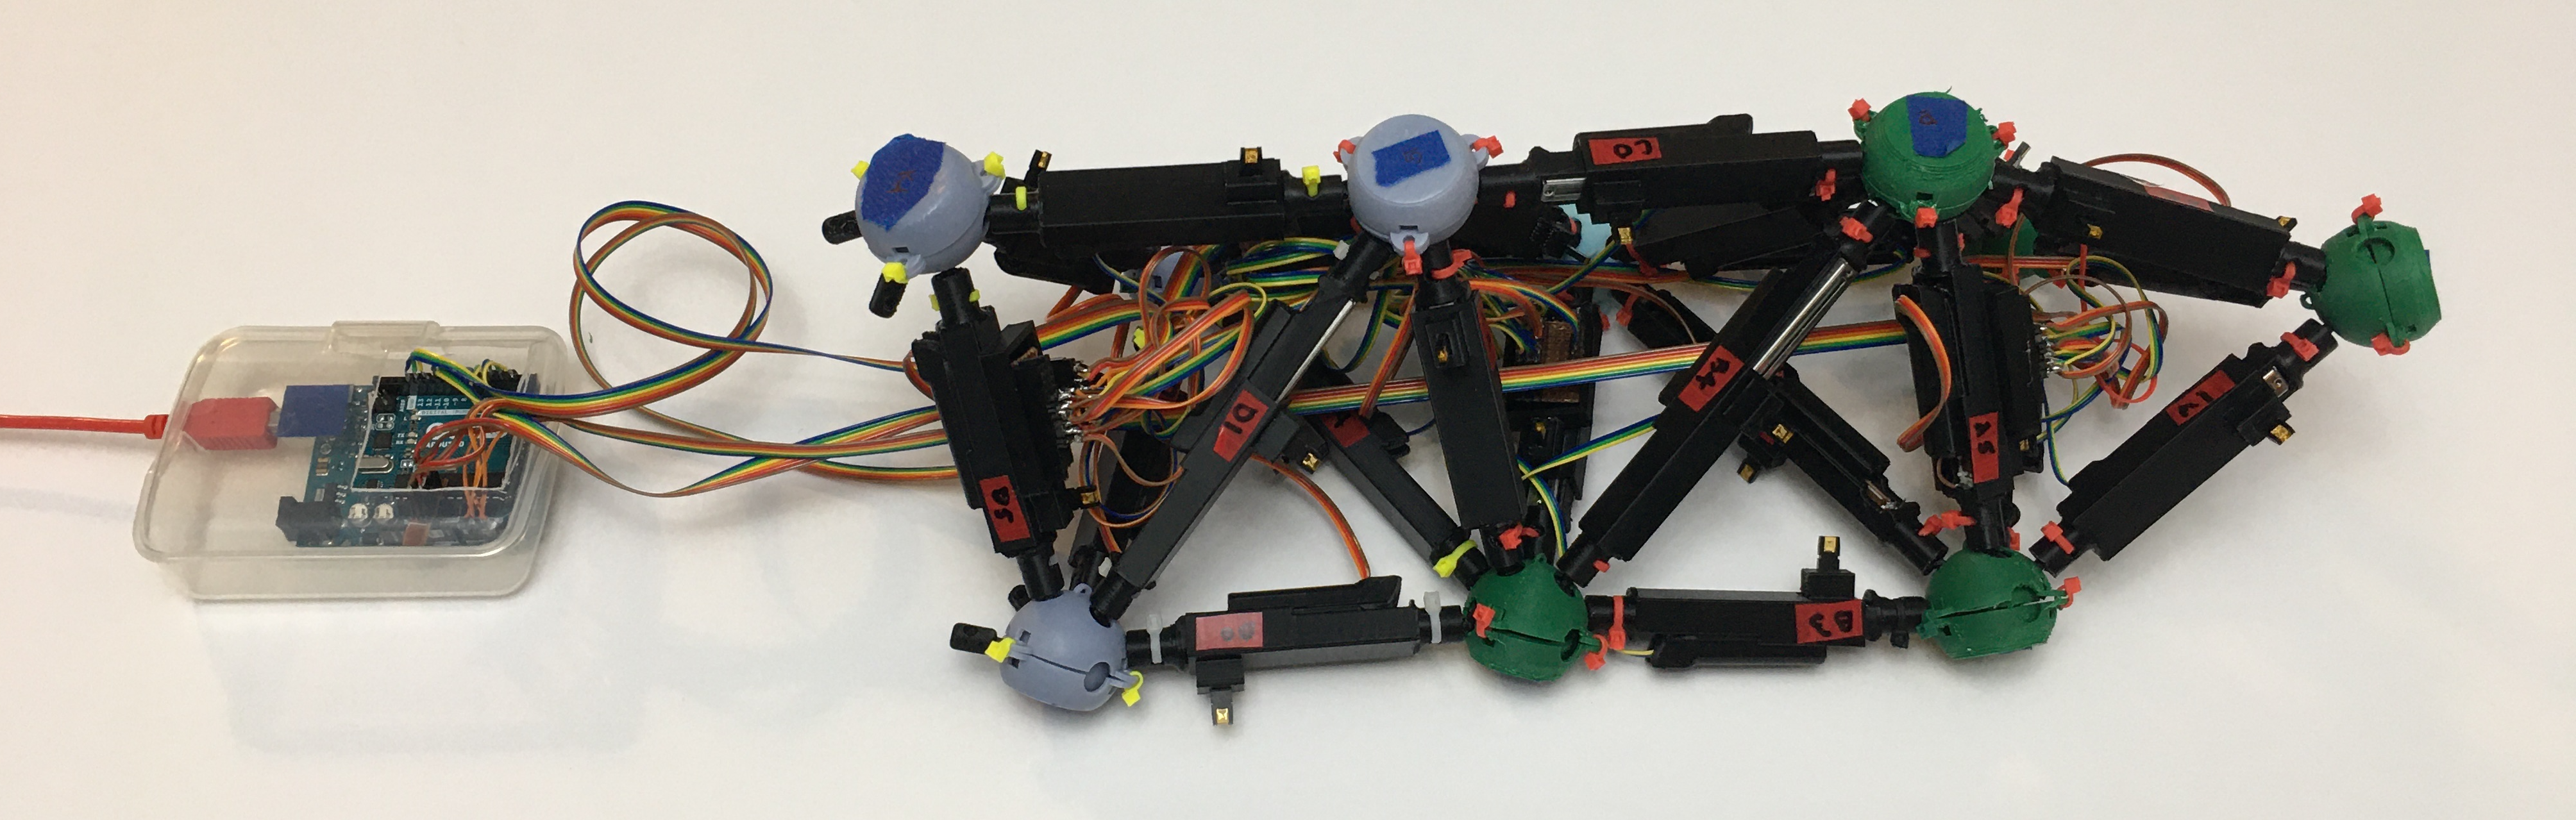
\includegraphics[width=0.5\textwidth]{figures/7TetControllerCropped.png}
    \caption[A 7-tetrahedron Controller]{A 7-tetrahedron Controller}
      \label{fig:7tetcontroller}
\end{figure}

\begin{figure}
  \centering
  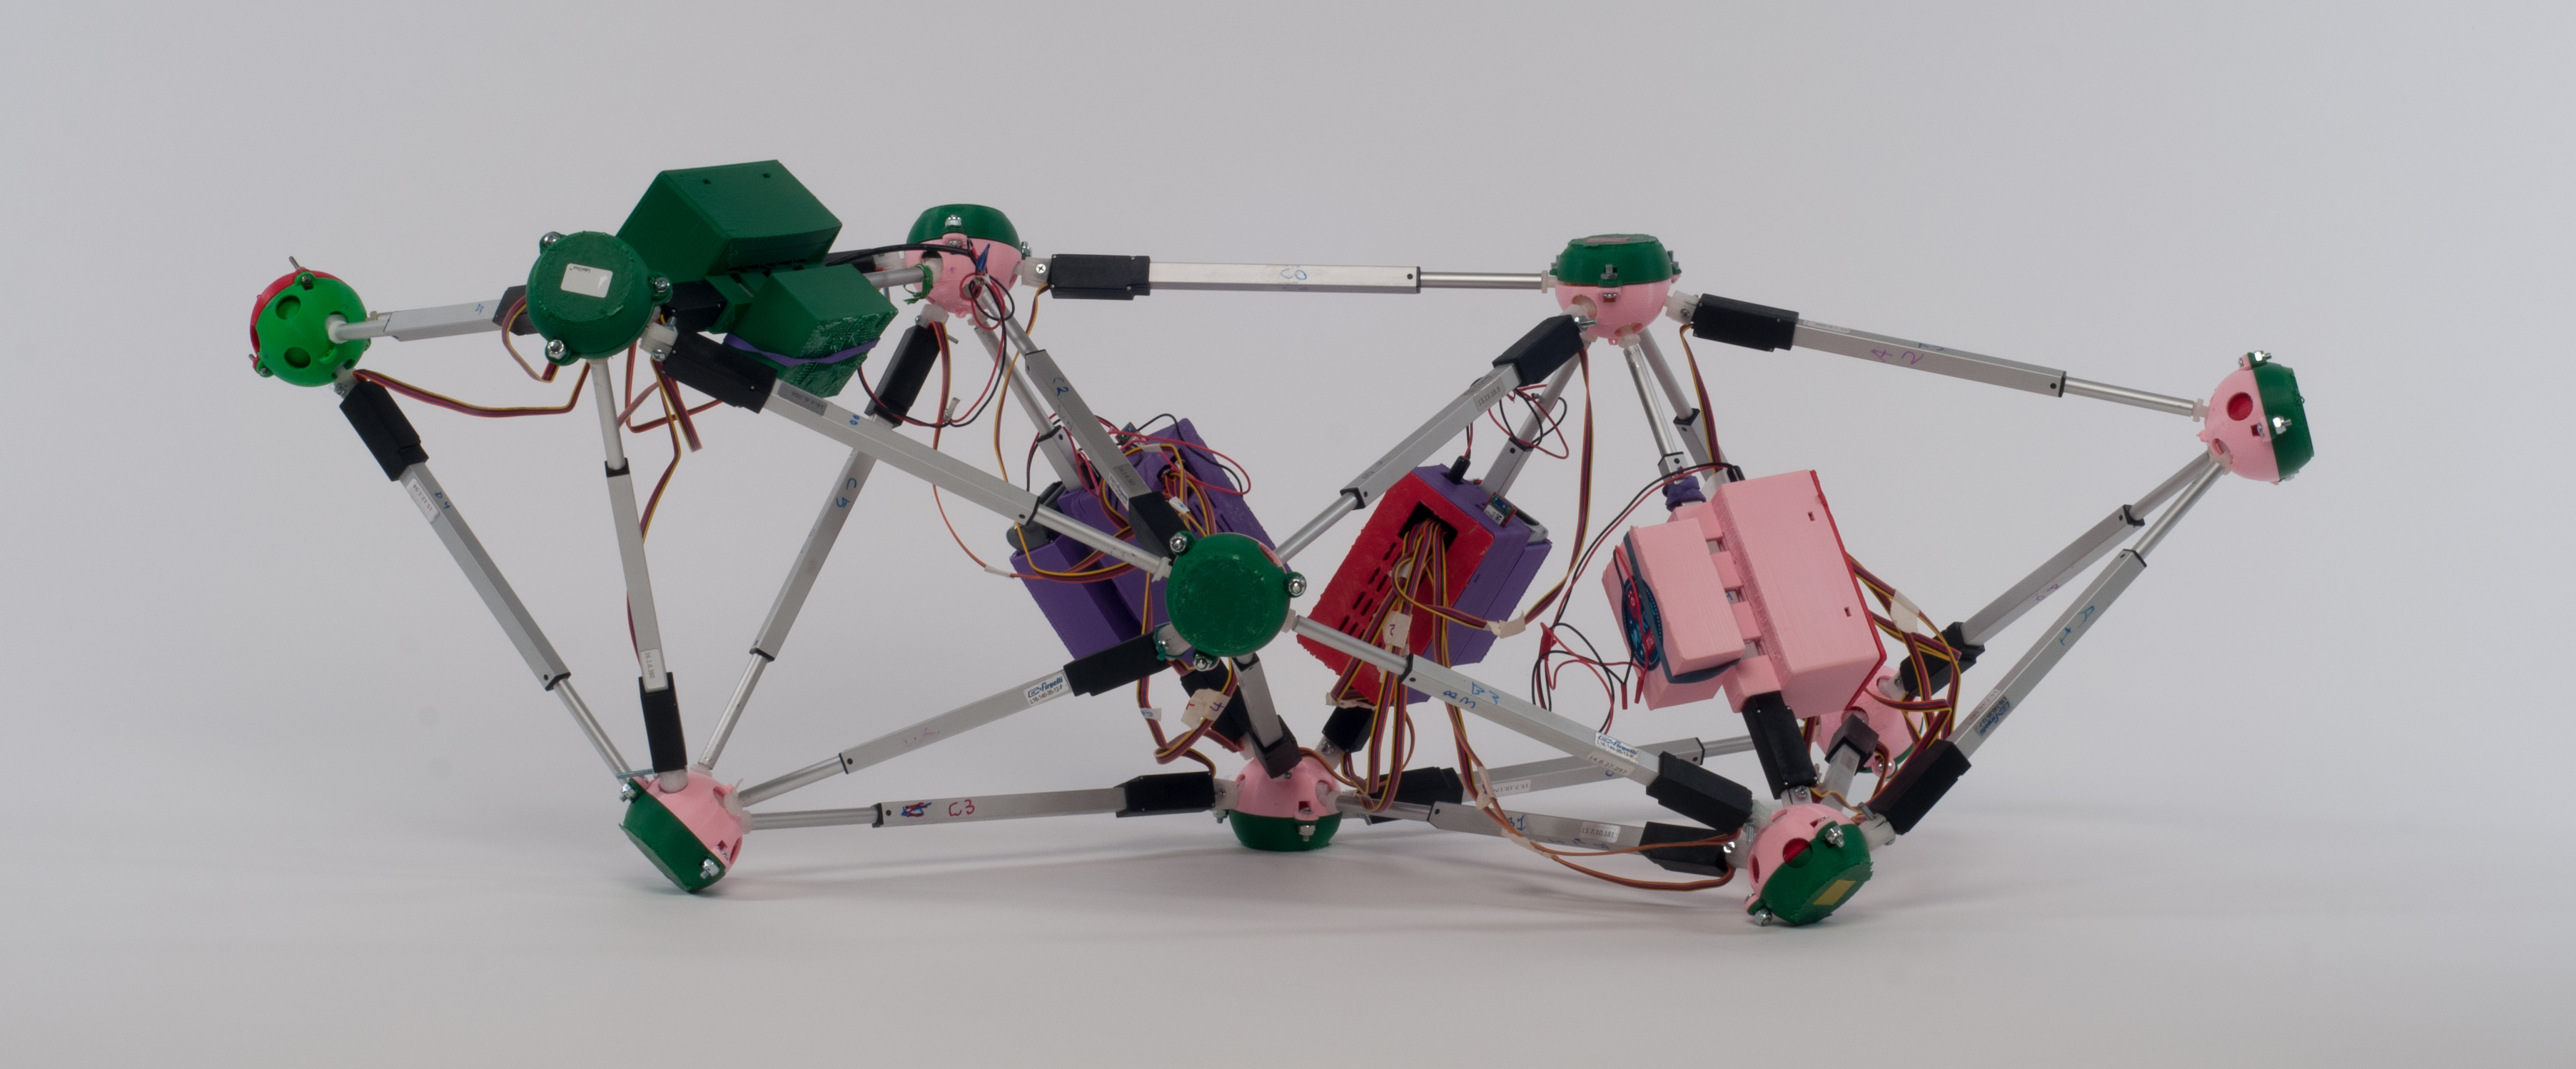
\includegraphics[width=0.5\textwidth]{figures/MedCantedCropped.png}
    \caption[A 7-tetrahedron Robot]{A 7-tetrahedron Tetrobot}
      \label{fig:7tetrobot}
\end{figure}



 \subsection{The Controller}

 The tetrocon device uses 3D printed Song-Kwon-Kim joints. The holes in
 the locking shell of this joint are centered so as to mimic a tetrahelix
 (slightly different configuration would be needed for other configurations.)
 So long as the ratio of maximum to minimum displacement of a member does not
 exceed the golden ratio ($\frac{\sqrt{5} + 1}/2$), the joint does moves
 freely and does not break.

 Linear potentiometers serve as linear dispacement sensors.
 These sensors are held in snap-together 3D printed sleeves, which have
 female parts to receive our universal jointing system. The entire
 system is modular, in the sense that every joint and
 every member is precisely the same.
 It snaps apart easily but is easy to repair.

 Because the controller is meant to be moved by hand through its range of
 operation with minial forces, we have found 3D-printed plastic parts acceptable,
 although occasional we have a layer sepration break with our rotors.

 Electronically, each of six potentiometers (forming a two-tetrahedra
 modular extention) is connected to a multiplexer, which controllers
 which signal is sent to an Arduino Uno microcontroller. This allows
 the 24 displacment sensors in a 7-tetrahedron controller to be
 digitized. A simple program returns all values upon request in
 JSON.

 A Python program implements a webserver, which allows other software
 to query the state of the 24 channels in the controller simply by
 making a web request.

 \subsection{The 7-Tet Tetrobot}

The 7-Tet Tetrobot, hereinafter simply called the tetrobot,
uses electromechanical actuators with a long lead screw driven by a small
rotary motor. The can exert 50 Newtons (11 pounds) of force, while weighing only a few hundred grams.

The tetrobot consists of four modules independent, each having (and carrying) a 12V NiMH battery, by far
the heaviest component of the robot. Thus in theory the tetrobot is expandable to any number of modules
while remaining untethered. Each modules control six actuators, so the addition of a new module adds
two more tetrahedra to the system. Each module has a Bluetooth radio on a custom Arduino Mega shield,
along with three two-channel motor controllers. The Arduino runs code which accepts commands to change
the length of members via Bluetooth. These commands are submitted by and Emacs electric lisp programmer,
making it convenient for an operator to issue commands in an Emacs lisp buffer.

The case to hold the battery and controller for each module is 3D printed with an orifice allowing
it to be mounted on the fixed part of an actuator.

In the tetrobot, the universal rotor is made by 3D printed steel ordered from Shapeways. Each
end of an actuator is bolted to an universal rotor. We attempted to attach the pushrod to the
universal rotor with a 3D printed plastic part, but found it necessary to move to an aluminum part.
A local machinist made the threaded pushrod connectors for us. The other end of the actuator is
larger and less prone to buckling forces, and we have so far been successful with plastic parts there.

The shell and ball of the Song-Kwon-Kim joint in fact is under very little force, and 3D printed
plastic parts have been acceptable. However, our current design requires the shell to be bolted
to a cap, and the bolts are prominent. When on the ground, they tend to catch and produce uneven
forces. We intend to move to a low-profile design soon.


 \section{Use of Controller with Tetrobot}

 \subsection{End-effector positioning}

 The simplest task for any robot that is capable of it is to position
 an end-effector in space. By orienting the tetrocon to match
 the physical position of the tetrobot, volunteers from an audience
 with zero experience can easily cause the first joint of the tetrobot
 to hit a positioned object after a few seconds of orientation.

 In a sesne this is a simulation of a robot ``arm'' that does not
 support locomotion.

 \subsection{Locomotion}

 A variable geometry truss wherein each element can change length
 has high input dimensionality; the 7-tet tetrobot has 24 actuators.
 The authors have previously explored developing gaits using a
 a virtual model of the tetrobot. This system used the ammo
 physics engine to simulate gravity. The basic goal to position
 six joints on the ground and then move one joint at a time,
 similar to a hexapodal gait on a robot with legs. Although
 some progress was made, the complexity of the software and
 physics simulation had many limitations.

 The controller, operating without the tetrobot,
 allowed us in a single hour to develop a set
 of thirteen positions which allows the robot to move forward
 on a smooth surface fairly effectively. As one might expect
 for a crawling robot, it was slow---approximately 4 inches
 per series of 13 poses, or approximately 4 inches per second
 (need to remeasuer precisely.)

 We also were able to create a set of poses that accomplished
 a 45 degree turn with the same ease. The tetrobot turns 45\degree in
 TBD minutes.

 However, when we were able to use the tetrobot with the tetrocon
 controller and see the effect of the robot position change directly
 within one or two seconds of changine the controller, we found we
 were much better able to intuitively develop motions for the robot.
 We discovered a more efficient ``inchworming'' gait which proved
 practical with two hours of experimentation. When recorded and
 replayed, this gait allows the tetrobot to move forward at TBD
 inches per minute.

 \subsection{Obstacle Confrontation}

 Unlike most wheeled vehicles and robots, the tetrobot might be able
 to climb over an obstacle of significant size compared to
 its own size. Operating in complex environments in a theoretic
 advantage of snake-like or tentacle-like robots.

 After successfully developing inchworming and turning gaits on
 flat terrain, we attacked the problem of climbing over a simple rectangular
 obstacle.  After practicing, we were able to manually control the
 tetrobot to climb over a 2''x2'' obstacle in TBD minutes. We then
 tested climbing over a 4''x4'' obstacle, and after TBD minutes of practice,
 were able to do it in TBD minutes. Finally, we attempted a 6''x6'' obstacle,
 and found TBD.

 \subsection{Summary of Locomotions}

\begin{table}[ht]
\caption{Locomotion Development} % title of Table
\centering % used for centering table
\begin{tabular}{c c c c} % centered columns (4 columns)
\hline\hline %inserts double horizontal lines
Locomotion & Practice Time & Motion Performance \\ [0.5ex] % inserts table
%heading
\hline % inserts single horizontal line
Inchworm Gait & 1.5 hours & X cm / minute \\ % inserting body of the table
Turn CW & 0.5 hours & X \degree / minute \\
Turn CCW & 0.5 hours & X \degree / minute \\
Cross 2x2 board & TBD hours & TBD minutes \\
Cross 4x4 board & TBD hours & TBD minutes \\
Cross 6x6 board & TBD hours & TBD minutes \\ [1ex] % [1ex] adds vertical space
\hline %inserts single line
\end{tabular}
\label{table:nonlin} % is used to refer this table in the text
\end{table}


 \section{Future Work: Virtual Control}

 Because the shape of a tetrahedron is completely determined by
 the length of its sides, it is possible to completely reconstruct
 the shape of the controller from its input. Software to do so
 is available on our site \citet{anonymous}.

 Becasue a tetrahelix is basically cylindrical or tentacle-like in
 shape, one can use the tetrocon to define a wide variety of shapes
 in space.  In fact the tetrocon supports a certain amount of size
 or thickenss information as well.  However, if valuable, you could
 consider only the centroid of each tetrahedron and thereby have
 a hand-manipulated specifier of curves in 3D Cartesian space.

 Thus any robot which is somewhat tentacle-like in shape could
 be controlled by the tetrocon. Since the tetrocon is modular,
 the length, in terms of the number of tetrahedra, is essentially
 unlimited. In practice, it becomes difficult to hold an object
 with too many tetrahedra. Our controller currently suffers
 from not offering enough resistance to change in displacemnt.
 That is, it is easy to move it into any position with the hands,
 but the potentiometers slide so easily that gravity may pull it
 back to the table of cause it to sag between your hands.

\section{Conclusion}
\label{sec:conclusion}

The use of a hand-manipulable controller that is the same shape
as the controlled robot allowed a complex tetrobot to be effectively
telepresently
controlled to develop programmable gaits and allowed a human
robot pilot to overcome obstacles with relative ease.

\section{Gait Speeds}
Inchworm:
Trial 0:
Node E begun on the starting line.
Time:  32.99 s
Travel: 12.5 cm

Trial 1:
Configuration resting configuration from inchworm.
Time: 34.17 s
Travel: 11 cm

Trial 2:
Time: 33.31
Travel: 11 cm

Conwalk:
Trial 0:
Node E begun on the starting line.
Time: 57.65
Travel: 10 cm

Trial 1:
Configuration resting configuration from inchworm.
Time: 55.04
Travel: 12 cm

Trial 2:
Time: 54.43
Travel: 6 cm : Note, locked against seam.

Tripod:
Trial 0:
Node E begun on the starting line.
Time: 57.65
Travel: 10 cm

Trial 1:
Configuration resting configuration from inchworm.
Time: 55.04
Travel: 12 cm

Trial 2:
Time: 54.43
Travel: 6 cm : Note, locked against seam.

Tripod:
Trial 1:
Time: 16.5 s
Travel: 6.5 cm

Trial 2:
Time: 16.85
Travel: 9 cm


6 steps 17.9 inches.




\section*{Acknowledgments}

Some people will be thanked after the anonymous review period.

%% Use plainnat to work nicely with natbib.

\bibliographystyle{plainnat}
\bibliography{references}

\end{document}






%\author{\authorblockN{Michael Shell}
%\authorblockA{School of Electrical and\\Computer Engineering\\
%Georgia Institute of Technology\\
%Atlanta, Georgia 30332--0250\\
%Email: mshell@ece.gatech.edu}
%\and
%\authorblockN{Homer Simpson}
%\authorblockA{Twentieth Century Fox\\
%Springfield, USA\\
%Email: homer@thesimpsons.com}
%\and
%\authorblockN{James Kirk\\ and Montgomery Scott}
%\authorblockA{Starfleet Academy\\
%San Francisco, California 96678-2391\\
%Telephone: (800) 555--1212\\
%Fax: (888) 555--1212}}


% avoiding spaces at the end of the author lines is not a problem with
% conference papers because we don't use \thanks or \IEEEmembership


% for over three affiliations, or if they all won't fit within the width
% of the page, use this alternative format:
%
%\author{\authorblockN{Michael Shell\authorrefmark{1},
%Homer Simpson\authorrefmark{2},
%James Kirk\authorrefmark{3},
%Montgomery Scott\authorrefmark{3} and
%Eldon Tyrell\authorrefmark{4}}
%\authorblockA{\authorrefmark{1}School of Electrical and Computer Engineering\\
%Georgia Institute of Technology,
%Atlanta, Georgia 30332--0250\\ Email: mshell@ece.gatech.edu}
%\authorblockA{\authorrefmark{2}Twentieth Century Fox, Springfield, USA\\
%Email: homer@thesimpsons.com}
%\authorblockA{\authorrefmark{3}Starfleet Academy, San Francisco, California 96678-2391\\
%Telephone: (800) 555--1212, Fax: (888) 555--1212}
%\authorblockA{\authorrefmark{4}Tyrell Inc., 123 Replicant Street, Los Angeles, California 90210--4321}}

\section{RSS citations}

Please make sure to include \verb!natbib.sty! and to use the
\verb!plainnat.bst! bibliography style. \verb!natbib! provides additional
citation commands, most usefully \verb!\citet!. For example, rather than the
awkward construction

{\small
\begin{verbatim}
\cite{kalman1960new} demonstrated...
\end{verbatim}
}

\noindent
rendered as ``\cite{kalman1960new} demonstrated...,''
or the
inconvenient

{\small
\begin{verbatim}
Kalman \cite{kalman1960new}
demonstrated...
\end{verbatim}
}

\noindent
rendered as
``Kalman \cite{kalman1960new} demonstrated...'',
one can
write

{\small
\begin{verbatim}
\citet{kalman1960new} demonstrated...
\end{verbatim}
}
\noindent
which renders as ``\citet{kalman1960new} demonstrated...'' and is
both easy to write and much easier to read.

\subsection{RSS Hyperlinks}

This year, we would like to use the ability of PDF viewers to interpret
hyperlinks, specifically to allow each reference in the bibliography to be a
link to an online version of the reference.
As an example, if you were to cite ``Passive Dynamic Walking''
\cite{McGeer01041990}, the entry in the bibtex would read:

{\small
\begin{verbatim}
@article{McGeer01041990,
  author = {McGeer, Tad},
  title = {\href{http://ijr.sagepub.com/content/9/2/62.abstract}{Passive Dynamic Walking}},
  volume = {9},
  number = {2},
  pages = {62-82},
  year = {1990},
  doi = {10.1177/027836499000900206},
  URL = {http://ijr.sagepub.com/content/9/2/62.abstract},
  eprint = {http://ijr.sagepub.com/content/9/2/62.full.pdf+html},
  journal = {The International Journal of Robotics Research}
}
\end{verbatim}
}
\noindent
and the entry in the compiled PDF would look like:

\def\tmplabel#1{[#1]}

\begin{enumerate}
\item[\tmplabel{1}] Tad McGeer. \href{http://ijr.sagepub.com/content/9/2/62.abstract}{Passive Dynamic
Walking}. {\em The International Journal of Robotics Research}, 9(2):62--82,
1990.
\end{enumerate}
%
where the title of the article is a link that takes you to the article on IJRR's website.


Linking cited articles will not always be possible, especially for
older articles. There are also often several versions of papers
online: authors are free to decide what to use as the link destination
yet we strongly encourage to link to archival or publisher sites
(such as IEEE Xplore or Sage Journals).  We encourage all authors to use this feature to
the extent possible.
